\documentclass{ctexart}
\usepackage{amsmath}
\usepackage{algorithm}
\usepackage{algorithmic}
\usepackage{amssymb}
\usepackage{amsthm}
\usepackage{bbm}
\usepackage{graphicx}
\usepackage{hyperref}
\newtheorem{lemma}{Lemma}
\newtheorem{theorem}{Theorem}
\newtheorem{remark}{Remark}
\DeclareMathOperator{\SIBM}{SIBM}
\DeclareMathOperator{\SSBM}{SSBM}
\DeclareMathOperator{\diag}{diag}
\DeclareMathOperator{\Var}{Var}
\DeclareMathOperator{\Bern}{Bern}
\DeclareMathOperator{\dist}{dist}
\DeclareMathOperator{\E}{\mathbb{E}}
\newcommand{\A}{\frac{a \log(n)}{n}}
\newcommand{\B}{\frac{b \log(n)}{n}}
\title{Exact recovery of Stochastic Block Model with Ising sampling}
\begin{document}
	\maketitle
	\section{Introduction}
	Based on Ising sampling, we propose a stochastic algorithm to achieve the exact recovery for stochastic block model (SBM).
	The stochastic algorithm can be transformed to an optimization problem, which includes maximum likelihood and maximal modularity.
	Besides, we give an unbiased convergent estimator of the parameters of SBM, which can be computed in constant time.
	Finally, we use metropolis sampling to realize the theoretical Ising sampling and demonstrates the better performance of our method,
	compared with other theoretically guaranteed algorithm.
	
	Stochastic Block Model (SBM) is one of statistical modeling for community detection problems.
	It provides benchmark artificial dataset to evaluate different community detection algorithms.
	Besides, SBM also inspires the design of algorithm for community detection tasks. These algorithms, such as
	semi-definite relaxation, spectral clustering and label propagation, not only have theoretical guarantee when applied to SBM,
	but perform well on dataset without SBM assumption. The study on the theoretical guarantee on SBM model can be divided between
	exact recovery and partial recovery. For both cases, the asymptotic behavior of detection error
	is analyzed when the scale of graph tends to infinity. There are already some well-known results of the exact recovery problem
	on SBM.	To name but a few, Abbe and Mossel established the exact recovery region for a special sparse SBM with two communities.
	Later on, the result is extended to general SBM with multiple communities.
	
	Besides theoretical study on SBM, in community detection maximal modularity is a popular detection method. The modularity is
	a kind of criteria and object function. By 
	\section{Stochastic Ising BlockModel}\label{sec:sibm}
	We consider a symmetric SBM model parameterized by $(n, k, p, q)$ where $p=\frac{a\log n}{n}, q=\frac{b\log n }{n}$.
	
	Let $W=\{1, \omega, \dots, \omega^{k-1}\}$ be a cyclic group with order $k$.
	Define an Ising model on a graph $G=([n],E(G))$ with parameters $\alpha,\beta>0$
	as the probability distribution on the configurations $\sigma\in W^n$ such that
	\begin{equation} \label{eq:isingma}
	P_{\sigma|G}(\sigma=\bar{\sigma})=\frac{1}{Z_G(\alpha,\beta)}
	\exp\Big(\beta\sum_{\{i,j\}\in E(G)} I(\bar{\sigma}_i ,\bar{\sigma}_j)
	-\frac{\alpha\log(n)}{n} \sum_{\{i,j\}\notin E(G)} I(\bar{\sigma}_i, \bar{\sigma}_j)\Big) ,
	\end{equation}
	where the subscript in $P_{\sigma|G}$ indicates that the distribution depends on $G$, and 
	$Z_G(\alpha,\beta)$
	is the normalizing constant. The indicator function is defined as
	$$
	I(x ,y) = \begin{cases}
	1 & x = y\\
	0 & x \neq y
	\end{cases}
	$$
	
	\section{Metropolis sampling algorithm for SIBM}
	In this section, we give an algorithm based on SIBM to do community detection tasks.
	For a SBM with $k-$communities, in previous section we have shown that the sample of SIBM is the same with the label $X$ up to some permutation. 
	Therefore, if we can get a sample from SIBM, then we can use this sample as the estimator of $X$.
	
	The difficulty is that we cannot generate the sample exactly from its distribution \eqref{eq:isingma}. Therefore, some approximation is
	necessary. The most common way to generate an Ising sample is using Metropolis sampling \cite{metropolis1953equation}.
	In this article, we use Metropolis sampling to generate SIBM sample.
	
	From equation \eqref{eq:isingma}, we know that for $k$-state Ising model, the Hamiltonian can be written as:
	\begin{equation}
	H(\bar{\sigma}) = \frac{\alpha}{\beta} \frac{\log n}{n} \sum_{\{i,j\}\not\in E(G)} \delta(\bar{\sigma}_i, \bar{\sigma}_j)
		- \sum_{\{i,j\}\in E(G)} \delta(\bar{\sigma}_i, \bar{\sigma}_j)
	\end{equation}
	Note: $\delta$ is the indicator function.
	
	Then Ising model generates sample according to $\exp(-\beta H(\bar{\sigma}))$. The physical meaning of $\beta$ is the inverse temperature.
	
	Suppose one coordinate $\bar{\sigma}_r$ flips to $w^s \cdot \bar{\sigma}_r$, the new state is denoted as $\bar{\sigma}^{(\sim \{r\}, v)}$.
	Then the change of energy is:
	\begin{equation}\label{eq:delta_H}
	 H(\bar{\sigma}^{(\sim \{r\}, [\omega^s])}) - H(\bar{\sigma}) = \sum_{i \in N_r(G)} J_s(\bar{\sigma}_r, \bar{\sigma}_i) - \frac{\alpha \log n}{\beta n} \sum_{i \in V\backslash N_r(G)\cup\{r\}} J_s(\bar{\sigma}_r,\bar{\sigma}_i)
	\end{equation}
	where $J_s(\sigma_i, \sigma_j)$ is defined as:
	\begin{equation}
	J_s(\sigma_i, \sigma_j) = \begin{cases}
	1 & \sigma_i = \sigma_j \\
	-1 & \omega^s \sigma_i = \sigma_j \\
	0 & \textrm {otherwise}
	\end{cases}
	\end{equation}
	\begin{remark}
	If we require $\bar{\sigma}_i \in \{\pm 1\}$ and use $\bar{\sigma}_i \cdot \bar{\sigma}_j$ replacing
	the indicator function  $\delta(\bar{\sigma},\bar{\sigma}_j)$ in \eqref{eq:delta_H}, the energy will be
	$$
	H(\bar{\sigma}) = \frac{\alpha}{\beta} \frac{\log n}{n} \sum_{\{i,j\}\not\in E(G)}\bar{\sigma}_i \cdot \bar{\sigma}_j
		- \sum_{\{i,j\}\in E(G)}\bar{\sigma}_i \cdot \bar{\sigma}_j
	 $$
	 suppose $\bar{\sigma}'$ is a state with one flop from $\bar{\sigma}$ at position $i$. That is
	 $$
	 \begin{cases}
	 \bar{\sigma}'_i &= -\bar{\sigma}_i \\
	 \bar{\sigma}'_j & = \bar{\sigma}_j \textrm{ for } j \neq i
	 \end{cases}
	 $$
	 Then the energy difference:
	 \begin{align}
	 H(\bar{\sigma}') - H(\bar{\sigma}) &= 2[\sum_{j\in N_i(G)}\bar{\sigma}_i \cdot \bar{\sigma}_j - \frac{\alpha \log n}{\beta n}
	 \sum_{\substack{j\not\in N_i(G) \\ j\neq i}} \bar{\sigma}_i \cdot \bar{\sigma}_j ] \notag\\
	 & = 2 [\sum_{j\in N_i(G)}(1+\frac{\alpha \log n}{\beta n})\bar{\sigma}_i \cdot \bar{\sigma}_j - \frac{\alpha \log n}{\beta n}
	 \sum_{j\neq i} \bar{\sigma}_i \cdot \bar{\sigma}_j ] \label{eq:energy_diff}
	 \end{align}
	 We use the conclusion that there are $\frac{n}{2} \bar{\sigma}_i$ takes value $1$ and $\frac{n}{2}\bar{\sigma}_i$ with value
	 $-1$. Therefore, $\sum_{j\neq i} \bar{\sigma}_i \cdot\bar{\sigma}_j = -1$.
	 
	 On the other hand:
	 $$
	 \frac{P_{\sigma | G}(\sigma = \bar{\sigma'})}{P_{\sigma | G}(\sigma = \bar{\sigma})}
	 = \frac{\exp(-\beta H(\bar{\sigma}'))}{\exp(-\beta H(\bar{\sigma}))} = \exp(-\beta(H(\bar{\sigma}')-H(\bar{\sigma})))
	 $$
	 By some simplification we can get the same result as \cite{ye2020exact} in Section III.A:
	 $$
	 \frac{P_{\sigma |G }(\sigma = X^{(\sim i)})}{P_{\sigma |G }(\sigma = X)}
	 = \exp(2(\beta + \frac{\alpha \log n}{n})(B_i - A_i)-\frac{2\alpha \log n}{n})
	 $$
	 For general cases, we consider sparse graph such that there are $O(\log n)$ neighbors for each node.
	 Also suppose that we store  attribute $m(\bar{\sigma})= |\{j \in [n], \bar{\sigma}_j = 1 \}|$.
	 Then \eqref{eq:energy_diff} reduces to:
	 \begin{equation}
	 H(\bar{\sigma}') - H(\bar{\sigma}) = 2 [\bar{\sigma}_i(1+\frac{\alpha \log n}{\beta n}) \sum_{j\in N_i(G)}\bar{\sigma}_j - \frac{\alpha \log n}{\beta n}
	 (\bar{\sigma}_i (2m-n)-1) ]
	 \end{equation}
	\end{remark}
	The pseudo code of our algorithm is summarized in \ref{alg:m}. This algorithm requires the number of the communities $k$ to be known and the weight parameter $\frac{\alpha}{\beta}$ is given. We use the annealing techniques (cooling temperature) to increase $\beta$ at each outer loop, thus guarantee that $\beta > \beta^*$
	if $\epsilon \in (0, 1)$ and $N$ are large. 
	The maximum iteration time $N$ should also be specified.
	\begin{algorithm}[H]
		\caption{Metropolis sampling algorithm for SIBM} \label{alg:m}
		Inputs: the graph $G$ \\
		Output: $\hat{X}$
		\begin{algorithmic}[1]
			\STATE random initialize $\sigma \in W^n$
			\WHILE{the iteration time $<N$}
			\FOR{each node $r$}
			\STATE random choose a new flipping state $w^s \cdot \sigma_r$
			\STATE compute $\Delta H(r,s) = H(\bar{\sigma}^{(\sim \{r\}, [w^s])}) - H(\bar{\sigma})$ using Equation \eqref{eq:delta_H}
			\IF{$\Delta H(r,s)<0$}
			\STATE $\sigma_r \leftarrow w^s \cdot \sigma_r$
			\ELSE
			\STATE generate a random number $u$ ranged within $[0,1]$
			\IF{$u < \exp(-\beta \Delta H(r,s))$}
			\STATE $\sigma_r \leftarrow w^s \cdot \sigma_r$
			\ENDIF
			\ENDIF
			\ENDFOR
			\IF{$H(\bar{\sigma})$ does not change}
			\STATE \textbf{break}
			\ENDIF
			\STATE $\beta \leftarrow (1 + \epsilon)\cdot\beta$
			\ENDWHILE
		\end{algorithmic}
	\end{algorithm}
	Since the computation of $\Delta H(r,s)$ needs $O(n)$ time. The time complexity of Algorithm \ref{alg:m} is $Nn^2$.
	\begin{remark}
	In the above scheme, we use the probability $\min\{1, \exp(-\beta \Delta H))\}$ for update. Another choice is to use
	the softmax (or Gibbs) probability to update. That is, the probability for position $r$ to transfer to state $\omega^s$ is
	$$
	P(\sigma_r \leftarrow \omega^s \cdot \sigma_r) = \frac{\exp(-\beta H(r, s))}{\sum_{r=0}^{k-1} \exp(-\beta H(r, s))}
	$$
	Instead of computing the energy term explicitly, we only need to compute the energy difference term:
	$$
	P(\sigma_r \leftarrow \omega^s \cdot \sigma_r) = \frac{\exp(-\beta \Delta H(r, s))}{\sum_{r=0}^{k-1} \exp(-\beta \Delta H(r, s))}
	$$
	where $\Delta H(r, 0) = 0$.
	If $k=2$ and $\Delta H = 0$, then it is equally likely to preserve the original state or flip its value. For Metropolis way it is
	definitely to flip its value.
	\end{remark}
	\section{error rate of SIBM}
	In the original article about SIBM \cite{ye2020exact}, it is not focused on the upper bound of error rate
	when exact recovery is (not) possible.
	Here we state the results in finer statement. We consider $k$ community directly.
	\begin{theorem}
		Let $\alpha > b \beta$,
		When $\beta > \beta^*$,
		$P_{\SIBM}(\sigma \not\in S_k(X)) \leq (2 + o(1)) n^{\tilde{g}(\beta)/4}$
	\end{theorem}
	\begin{proof}
		We only need to show that $P_{\SIBM}(\sigma \neq X | D(\sigma, X)) \leq (2 + o(1)) n^{\tilde{g}(\beta)/4}$
		Since $P_{\SIBM}(\sigma \neq X | D(\sigma, X)) = P_{\SIBM}(\sigma \neq X, \dist(\sigma, X) \leq n/\log^{\delta}(n)  | D(\sigma, X))
		+ P( \dist(\sigma, X) > n/\log^{\delta}(n) | D(\sigma, X))$.
		For the second term, it is controlled by:
		$P( \dist(\sigma, X) > n/\log^{\delta}(n) | D(\sigma, X))< n^{-C}$ for any $C>0$.
		For the first term, we have
		$P_{\SIBM}(\sigma \neq X, \dist(\sigma, X) \leq n/\log^{\delta}(n)  | D(\sigma, X)) =
		P_{\SIBM}(\sigma \neq X  |  \dist(\sigma, X) \leq n/\log^{\delta}(n) ) P_{\SIBM}( \dist(\sigma, X) \leq n/\log^{\delta}(n) | D(\sigma, X))
		\leq P_{\SIBM}(\sigma \neq X  |  \dist(\sigma, X) \leq n/\log^{\delta}(n) )$
		$$
		P_{\SIBM}(\sigma \neq X  |  \dist(\sigma, X) \leq n/\log^{\delta}(n) )
		= \sum_{G\in G'} P_G(G)P_{\sigma |G }(\sigma \neq X  |  \dist(\sigma, X) \leq n/\log^{\delta}(n) ) + P(G'^c)
		$$
		where $P(G'^c) \leq \frac{2 n^{\tilde{g}(\beta)/4}}{1-n^{\tilde{g}(\beta)/4}}$.
		$$
		P_{\sigma | G}(\sigma \neq X  |  \dist(\sigma, X) \leq n/\log^{\delta}(n) ) 
		= \sum_{r=1}^{n/\log^{\delta}(n)} P_{\sigma | G}(\dist(\sigma, X) = r |  \dist(\sigma, X) \leq n/\log^{\delta}(n) ) 
		$$
		Let $\ell = \sum_{r=1}^{n/\log^{\delta}(n)} P_{\sigma | G}(\dist(\sigma, X) = r |  \dist(\sigma, X) \leq n/\log^{\delta}(n) ) $
		Since
		$$
		\frac{\ell}{1-\ell} = \frac{\ell}
		{P_{\sigma | G}(\sigma = X |  \dist(\sigma, X) \leq n/\log^{\delta}(n) ) } \leq \frac{n^{\tilde{g}(\beta)/2}}{1-n^{\tilde{g}(\beta)/2}}
		$$
		$\ell \leq n^{\tilde{g}(\beta)/2}$.
		Therefore, the dominate term is $2n^{\tilde{g}(\beta)/4}$
	\end{proof}
\begin{remark}
	We can further enhance the result to
	$$
	P_{\SIBM}(\sigma \not\in S_k(X)) \leq (1 + o(1)) n^{\tilde{g}(\beta)/2}
	$$
\end{remark}
	\section{Parameter Estimation for SBM}
	In Section \ref{sec:sibm}, we have shown that when $\alpha > b \beta$ and $\beta > \beta^*$. The sample of SIBM aligns with $X$ with probability one
	as $n\to \infty$. 
	% conjecture, both alpha and beta cannot be too large, otherwise the convergence of Metropolis sampling is very slow.
	The critical value $\beta^*$ is a function of $a$ and $b$. Therefore, to give good guarantee of Algorithm \ref{alg:m}, we need to estimate the parameter
	of $a,b$ before estimating the label of $X$.
	This estimation is done by counting the edges and triangles of the input graph $G$.
	Since the graph is random, the number of edges $T_1$ is also a random variable and its expectation is
	\begin{equation}
	E[T_1] = k \frac{n/k(n/k-1)}{2} p + \frac{k(k-1)}{2} (n/k)^2 q \sim \frac{n\log n}{2k} (a + (k-1) b)
	\end{equation}
	When $n \to \infty$ by the law of large numbers we can show that $\frac{T_1}{n \log n}$ converges to $\frac{a+(k-1)b}{2k}$ in probability.
	
	Similarly, for the number of triangles $T_2$ we can compute its expectation as:
	\begin{align}
	E[T_2] &= k \frac{n/k(n/k-1)(n/k-2)}{6}p^3 + 2\frac{k(k-1)}{2}(n/k) \frac{n/k(n/k-1)}{2} pq^2 + \binom{k}{3} \left(\frac{n}{k}\right)^3 q^3 \\
	&\sim \frac{(\log n)^3}{k^2}
	(\frac{a^3}{6} + \frac{k-1}{2}ab^2 + (k-1)(k-2)\frac{b^3}{6})
	\end{align}
	When $n$ is large, we can also show that $\frac{T_2}{(\log n)^3}$ converges to $\frac{1}{k^2}
	(\frac{a^3}{6} + \frac{k-1}{2}ab^2)$. Therefore we can get the equation array about $a$ and $b$:
	\begin{align}
	\frac{a+(k-1)b}{2k} & = e_1 \label{eq:e_1}\\
	\frac{1}{k^2}
	\left(\frac{a^3}{6} + \frac{k-1}{2}ab^2 + (k-1)(k-2)\frac{b^3}{6}\right) & = e_2 \label{eq:e_2}
	\end{align}	
	
	Solving this equation and use the assumption that $ a > b, 0 < a < e_1$ we can get the unique solution of $(a,b)$.
	This is our parameter estimation method.
	\section{Connection with Modularity Based Method}
	To simplify our analysis, we consider $k=2$ in this section. Our conclusion is that for SBM with large $n$, modularity method
	is a special model of SIBM. The $\alpha, \beta$ are fixed values, which is not optimal for the specific SBM problem. We use theoretical
	analysis and simulation to verify our declaration.

	Now we compute modularity for SBM$(n,k, a\frac{\log n}{n}, b\frac{\log n}{n})$.
	The standard formula is
	\begin{equation}
	Q = \frac{1}{2m} \sum_{ij} (A_{ij} - \frac{d_i d_j}{2m}) \delta(C_i, C_j)
	\end{equation}
	The standard way to do community detection is to maximize the modularity $Q$ using greedy method.
	Suppose we use $Q$ in the definition of the numerator of Ising model. When $n$ is very large,
	we have $d_i = \frac{\log n(a+b)}{2}, m = \frac{1}{2}n d_i$. Therefore we have $\beta = \frac{1}{2m}(1-\frac{\log n}{2n}(a+b))
	\sim \frac{1}{2m}$
	and $\alpha = \frac{1}{2m}\frac{a+b}{2}$. Since $a>b$. We have $\alpha > b \beta$, which is a necessary condition for finite sample complexity.
	However, due to the scaling effect, we can not get the conclusion on the critical value $\beta^*$.
	
	When $\alpha > b \beta$, we can do an optimization problem:
	\begin{align}\label{eq:opsig}
	\max_{\sigma} \,\,& \beta \sum_{\{i,j\} \in E(G)} \sigma_i \sigma_j - \frac{\alpha \log n}{n} \sum_{\{i,j\} \in E(G)} \sigma_i \sigma_j\\
	s.t. \,\, & \sigma \in \{\pm 1\}^n
	\end{align}
	If the above equation can be solved exactly, then the solution is the true label with probability 1 as $n\to \infty$.
	
	This fact is easy to show using SIBM theory. we can always scaling the object function such that $\beta > \beta^*$.
	Then the sample from SIBM is $\pm X$ with probability 1 and it is equivalent to do the above optimization problem.
	This conclusion also verifies that Modularity maximization method is asymptotic optimal for SBM.
	
	For the given optimization problem in Equation \eqref{eq:opsig}, we can let $\beta = 1$ as given for modularity maximization method (we omit the scaling term $\frac{1}{2m}$).
	Then our condition is $\alpha > b$. The choice of $\alpha$ for modularity method is $\frac{a+b}{2}$. We want to
	investigate whether this choice is optimal for some approximation solution of modularity maximization.
	
	We can use simulation annealing to search for the optimal value of Equation \eqref{eq:opsig}. This method has been tried
	by \cite{he2016fast}. The earliest literature for adoption is \cite{liu2010detecting}, empirically combined with other techniques to improve
	the performance.
	\section{SDP Algorithms Proofs}
\begin{lemma}\label{lem:Cabd}
	Let $e_n$ be the all-one vector with length $n$.
	Suppose $C$ is a following symmetric matrix.
	$$
	C= \begin{bmatrix}
C_1 & C_2 \\
C_2^T & C_3 \\
\end{bmatrix},	
C_1=
\begin{bmatrix} d & \text{ } &  a \\
\text{ } & \ddots & \text{ } \\
a & \text{ } & d 
\end{bmatrix},
C_3=
\begin{bmatrix} c & \text{ } &  a \\
\text{ } & \ddots & \text{ } \\
a & \text{ } & c
\end{bmatrix}
$$
and $C_2 = b e_n e_m^T$, $\dim(C_1) = n \times n, \dim(C_3) = m \times m$.
then the characteristic polynomial function is
$$
p(\lambda) = 
(\lambda - d + a)^{n-1} (\lambda - c + a)^{m-1}
[(\lambda - d - (n-1)a)
 (\lambda - c - (m-1)a)
- nmb^2]
$$
 
 A special case is $d=c,m=n$, then $d + (n-1)a+ nb$ corresponds to the all-one eigenvector while 
 $d +(n-1)a -nb$ corresponds to the eigenvector $g=(1,\dots, 1, -1, \dots, -1)$.
\end{lemma}
\begin{proof}
Let $d' = d-a, c'=c-a$,
then the matrix $\lambda I_{n+m} - C$ can be written in block form:
$$
\lambda I_{n+m} - C = \begin{bmatrix}
(\lambda -d') I_n - a e_ne_n^T & -b e_ne_m^T \\
-be_me_n^T & (\lambda -c') I_m - a e_me_m^T
\end{bmatrix}
$$
Using Woodbury matrix inverse we can compute
$$
[(\lambda -c') I_m - a e_me_m^T]^{-1} = (\lambda - c')^{-1} [I_m - \frac{a}{ma - \lambda + c'} e_me_m^T]
$$
Using the block matrix formula for determinate, i.e.
$$
\begin{vmatrix}
A & B \\
C & D
\end{vmatrix} = |D| \times |A-BD^{-1}C|
$$
we further have
$$
|\lambda I_{n+m} - C| = |(\lambda -c') I_m - a e_me_m^T| |(\lambda - d')I_n + \kappa e_ne_n^T|
$$
where
\begin{align*}
\kappa &= -a - \frac{b^2}{\lambda - c'} e_m^T (I_m - \frac{a}{ma-\lambda + c'}e_me_m^T)e_m \\
&= -a  - \frac{b^2 m}{\lambda - ma - c'}
\end{align*}
Further for matrix of the form $(x-y)I_n + yee^T$, its determinant can be computed explicitly
as $|(x-y)I_n + yee^T|=(x-y)^{n-1}(x+(n-1)y)$ (See Example 1.5.9 of \cite{ad_li}.)
Or equivalently, $|zI_n + yee^T|=z^{n-1}(z+ny)$.
Therefore, we can finally get the characteristic function:
$$
|\lambda I_{n+m} - C| = (\lambda -c')^{m-1}(\lambda -d')^{n-1}  [(\lambda - d' - na)(\lambda - c' - ma)-nmb^2]
$$
\end{proof}
\begin{lemma}\label{lem:Cabd2}
	Suppose $C$ is a following symmetric matrix with dim = $kn$.
	$A, B$ is a matrix with dim = $n$
	$$A=\begin{bmatrix}
	d & \text{ } & a \\
	& \ddots & \\
	a & \text{ } & d 
	\end{bmatrix},
	B=\begin{bmatrix}
	b & \text{ } & b \\
	& \ddots & \\
	b & \text{ } & b 
	\end{bmatrix},
	 C=\begin{bmatrix} 
	 	A & \text{ } & B \\
	 & \ddots & \\
	 B & \text{ } & A 
	\end{bmatrix}$$,
	then the characteristic polynomial function of $C$ is $(\lambda - d + a)^{kn-k} (\lambda - d - (n-1)a + nb)^{k-1}
	(\lambda - d - (n-1)a -(k-1)nb)$. $d + (n-1)a + (k-1)nb$ corresponds to the all-one eigenvector.
\end{lemma}
\section{Proofs of Parameter Estimation}
	\begin{lemma}
		Suppose $e_1, e_2$ is defined from (\ref{eq:e_1}, \ref{eq:e_2}), Then the following equation array has unique solution $x=a, y=b$
		\begin{align}
	\frac{x+(k-1)y}{2k} & = e_1 \\
\frac{1}{k^2}
\left(\frac{x^3}{6} + \frac{k-1}{2}xy^2 + (k-1)(k-2)\frac{y^3}{6}\right) & = e_2	
		\end{align}
	\end{lemma}
\begin{proof}
	Using $x=2ke_1 - (k-1)y$ we can get
	\begin{equation}
	g(y): = (k-1)(y^3 - 6 e_1 y^2 + 12 e_1^2 y) + 6 e_2 - 8 k e_1^3 = 0
	\end{equation}
	This equation has unique real root since $g(y)$ is increasing on $\mathbb{R}$. $g'(y) = 3(k-1)(y-2e_1)^2 \geq 0 $
	Next we show the root lies within $(0, 2e_1)$.
	\begin{align*}
	g(0) &= \frac{1}{k^2}\left(-3(k-1)(k-2)ab^2 + (k-1)((k-2)-(k-1)^2)b^3\right) < 0 \\
	g(2e_1) &= 6e_2 - 8e_1^3 = \frac{(k-1)(a-b)^3}{k^3} > 0
	\end{align*}
	Therefore, we can get a unique solution $y$ within $(0, 2e_1)$. Since $(a,b)$ is a solution for the equation array. The conclusion follows.
	
\end{proof}
	\begin{lemma}\label{lem:ERT}
	In an ER graph parameterized by $(n,p)$ and $p=\frac{a\log n}{n}$, the number of edges is denoted by $T(G)$, then
	$\frac{T}{n \log n} \to \frac{a}{2}$ in probability.
	% Erdős–Rényi
	\end{lemma}
\begin{proof}
	Let $X_{ij}$ represents a Bernoulli random variable with parameter $p$. Then $T(G) = \sum_{i,j} X_{ij}$, $X_{ij}$ are i.i.d.
	$E[T(G)] = \frac{n(n-1)}{2}p = \frac{(n-1)\log n}{2}a$ and $\Var[T(G)] = \frac{n(n-1)}{2} p(1-p) < a\frac{(n-1)\log n}{2}$
	Then by Chebyshev's inequality
	$$
	\Pr(\Big|\frac{T}{n \log n } - \frac{a}{2} \frac{n-1}{n}\Big| > \epsilon) \leq \frac{\Var[T /(n \log n )]}{\epsilon^2} < \frac{a(n-1)}{2n^2\epsilon^2\log n}
	$$
	For a given $\epsilon$, when $n$ is sufficiently large,
	$$
	\Pr(\Big|\frac{T}{n \log n } - \frac{a}{2} \Big| > \epsilon) < \Pr(\Big|\frac{T}{n \log n } - \frac{a}{2} \frac{n-1}{n}\Big| > 2\epsilon)
	\leq \frac{n-1}{8n^2 \epsilon^2 \log n}
	$$
	Therefore, by the definition of convergence in probability, we have $\frac{T}{n \log n} \to \frac{a}{2}$ as $n\to \infty$.
\end{proof}
\begin{lemma}\label{lem:ER_tr_counting}
	In an ER graph parameterized by $(n,p)$ and $p=\frac{a\log n}{n}$, the number of triangles is denoted by $T(G)$, then
	$\frac{T}{(\log n)^3} \to \frac{a^3}{6}$ in probability.
	% Erdős–Rényi
\end{lemma}
\begin{proof}
	Let $X_{ijk}$ represents a Bernoulli random variable with parameter $p^3$.
	Then $T(G) = \sum_{i,j,k} X_{ijk}$.
	It is easy to compute that $E[T] = \binom{n}{3}p^3$.
	From \cite{holland1977method} we know that
	% Mordern version: https://stats.stackexchange.com/questions/338267/distribution-and-variance-of-count-of-triangles-in-random-graph
	$$
	\Var[T] = \binom{n}{3} p^3 + 12 \binom{n}{4} p^5 + 30 \binom{n}{5} p^6 + 20 \binom{n}{6} p^6 - \binom{n}{3}^2 p^6 = O(\log^3 n)
	$$
	Therefore
	by Chebyshev's inequality
	$$
	\Pr(\Big|\frac{T}{\log^3 n } - \frac{a^3}{6} \frac{(n-1)(n-2)}{n^2}\Big| > \epsilon) \leq \frac{\Var[T /\log^3 n ]}{\epsilon^2} 
	= \frac{1}{\epsilon^2}O(\frac{1}{\log^3 n})
	$$
	Similar to Lemma \ref{lem:ERT} we can show that the convergence of $\frac{T}{\log^3 n}$ to $\frac{a^3}{6}$.
\end{proof}
\begin{lemma}\label{lem:SBM_tr_counting_cross}
	Consider a 2 community SBM $(2n, p, q)$ and count the number of triangles $T$ which has a node in $S_1$ and an edge in $S_2$.
	Then the variance of $T$ is
	\begin{equation}\label{eq:SBM_tr_counting_cross}
	\Var[T] = \frac{n^2(n-1)}{2}q^2p + n^2(n-1)(n-2)p^2q^3 +\frac{n^2(n-1)^2}{2}q^4p - \frac{n^2(n-1)(3n-4)}{2}q^4 p^2
	\end{equation}
\end{lemma}
\begin{proof}
	$T=\sum_{i,j,k} Y_{ijk}$ where the summation is over $i \in S_1$ and $j,k \in S_2$. Therefore, $E[T] = n\binom{n}{2}pq^2$
	To compute the variance of $T$ we need to compute $E[T^2] = \sum_{i,j,k}\sum_{i',j',k'} Y_{ijk}Y_{i'j'k'}$.
	There are 6 cases for $E[Y_{ijk}Y_{i'j'k'}]$
	\begin{enumerate}
		\item $\{i,j,k\} = \{i',j',k'\}$ then $E[Y_{ijk}Y_{i'j'k'}] = pq^2$.
		There are $n\binom{n}{2}$ such terms in the double sum.
		\item If $\{i,j,k\}$ and $\{i',j',k'\}$ have exactly 1 element in common and the element $\in S_1$, then $E[Y_{ijk}Y_{i'j'k'}] = p^2q^4$.
		There are $6n\binom{n}{4}$ such terms in the double sum. ($\binom{4}{2}=6$)
		\item If $\{i,j,k\}$ and $\{i',j',k'\}$ have exactly 1 element in common and the element $\in S_2$, then $E[Y_{ijk}Y_{i'j'k'}] = p^2q^4$.
		There are $12\binom{n}{2}\binom{n}{3}$ such terms in the double sum.
		\item If $\{i,j,k\}$ and $\{i',j',k'\}$ have exactly 2 elements in common and the two elements are both $\in S_2$, then $E[Y_{ijk}Y_{i'j'k'}] = pq^4$.
There are $2\binom{n}{2}\binom{n}{2}$ such terms in the double sum.
\item If $\{i,j,k\}$ and $\{i',j',k'\}$ have exactly 2 elements in common and one is in $S_1$, the other is in $S_2$, then $E[Y_{ijk}Y_{i'j'k'}] = p^2q^3$.
There are $6n\binom{n}{3}$ such terms in the double sum.
\item If $\{i,j,k\}$ and $\{i',j',k'\}$ have 0 element in common, then $E[Y_{ijk}Y_{i'j'k'}] = p^2q^4$.
There are $12\binom{n}{2}\binom{n}{4}$ such terms in the double sum.
	\end{enumerate}
To verify we have covered all cases, note that the sum adds up to $(n\binom{n}{2})^2$:
% Mathematica Code:
% Simplify[n^2 (n-1)/2 + 12 Binomial[n,2] Binomial[n,3] + 6 n Binomial[n,4] + Binomial[n,4] Binomial[n,2]*12 + 6 n Binomial[n,3]+ 2 Binomial[n,2]^2]
$$
n\binom{n}{2} + 6n\binom{n}{4} + 12\binom{n}{2} \binom{n}{3} + 2(\binom{n}{2})^2 + 6n\binom{n}{3} + 12\binom{n}{2}\binom{n}{4} = \left(n\binom{n}{2}\right)^2
$$
\end{proof}
\begin{lemma}\label{lem:SBM_tr_counting_3}
	Consider a 3 community SBM$(3n, p, q)$ and count the number of triangles $T$ which has a node in $S_1$, one node in $S_2$ and one node in $S_3$.
	Then the variance of $T$ is
	\begin{equation}\label{eq:SBM_tr_counting_three}
	\Var[T] = n^3 q^3  + 3n^3(n-1) q^4  + 3 n^3 (n-1)^2 q^5 - n^3(3n^2-3n+1)q^6
	\end{equation}
\end{lemma}
\begin{proof}
	Similar to Proof of Lemma \ref{lem:SBM_tr_counting_cross}.
	$E[T] = n^3 q^3$ and there are 4 cases
	\begin{enumerate}
	\item $\{i,j,k\} = \{i',j',k'\}$ then $E[Y_{ijk}Y_{i'j'k'}] = q^3$.
	There are $n^3$ such terms in the double sum.
	\item If $\{i,j,k\}$ and $\{i',j',k'\}$ have exactly 1 element in common, then $E[Y_{ijk}Y_{i'j'k'}] = q^5$.
	There are $12n\binom{n}{2}^2$ such terms in the double sum.
	\item If $\{i,j,k\}$ and $\{i',j',k'\}$ have exactly 2 element in common, then $E[Y_{ijk}Y_{i'j'k'}] = q^4$.
	There are $6\binom{n}{2}n^2$ such terms in the double sum.
	\item If $\{i,j,k\}$ and $\{i',j',k'\}$ have 0 element in common, then $E[Y_{ijk}Y_{i'j'k'}] = q^6$.
	There are $8\binom{n}{2}^3$ such terms in the double sum.		
\end{enumerate}	
To verify we have covered all cases, note that the sum adds up to $n^6$:
$$
6(\binom{n}{2})n^2  + 8(\binom{n}{2})^3 + 12n(\binom{n}{2})^2 +  n^3 = n^6
$$
\end{proof}
\begin{theorem}
	For a SBM$(n, k, p, q)$ where $p=\frac{a\log n}{n}, q = \frac{b\log n}{n}$. The number of triangles is $T$.
	Then $\frac{T}{(\log n)^3}$ converges to $\frac{1}{k^2}(\frac{a^3}{6} + \frac{k-1}{2}ab^2 + (k-1)(k-2)\frac{b^3}{6} )$ in probability as $n \to \infty$.
\end{theorem}
\begin{proof}
	We split $T$ into three parts, the first is the number of triangles within community $i$, $T_i$. There are $k$ terms of $T_i$.
	The second is the number of triangles which have one node in community $i$ and one edge in community $j$, $T_{ij}$. There are $k(k-1)$ terms of $T_{ij}$. The third is the number of triangles which have one node in community $i$, one node in community $j$ and one node in community $k$.
	
	We only need to show that
	\begin{align}
	\frac{T_i}{\log ^3 n} &\to \frac{(a/k)^3}{6} \\
	\frac{T_{ij}}{\log^3 n}& \to \frac{1}{2}(a/k)(b/k)^2\\
	\frac{T_{ijk}}{\log^3 n} & \to (b/k)^3
	\end{align}
	The convergence of $\frac{T_i}{\log ^3 n}$ comes from Lemma \ref{lem:ER_tr_counting}.
	For $T_{ij}$ we use the conclusion from Lemma \ref{lem:SBM_tr_counting_cross}.
	We replace $n$ with $n/k$, $p=a\frac{\log n}{n}$, $q=b\frac{\log n}{n}$ in Equation \eqref{eq:SBM_tr_counting_cross}.
$\Var[T_{ij}] \sim \frac{ab^2}{2k^3} \log^3 n$. Since the expectation of $\frac{T_{ij}}{\log^3 n}$ is $(n/k)\binom{n/k}{2}pq^2/(\log^3 n)
=\frac{n-1}{2n}\frac{ab^2}{k^3}$. By Chebyshev's inequality we can show that 
\begin{align*}
P( \Big|\frac{T_{ij}}{\log^3 n} - \frac{n-1}{2n}\frac{ab^2}{k^3} \Big| > \epsilon) &\leq \frac{\Var[T_{ij} / \log^3 n]}{\epsilon^2} \\
& = \frac{1}{\epsilon^2}
O(\frac{1}{\log^3 n})
\end{align*}
	Therefore, $\frac{T_{ij}}{\log^3 n} $ converges to $\frac{1}{2}(a/k)(b/k)^2$
	
	To prove $\frac{T_{ijk}}{\log^3 n}\to (b/k)^3$, from Lemma \ref{lem:SBM_tr_counting_3} we can get $\Var[T_{ijk}] = O(\log^5 n)$
$$
\Pr( \Big|\frac{T_{ijk}}{\log^3 n} -\frac{b^3}{k^3} \Big| > \epsilon) \leq \frac{\Var[T_{ijk} / \log^3 n]}{\epsilon^2} = \frac{1}{\epsilon^2}
O(\frac{1}{\log n})
$$
\end{proof}
\section{SDP for two community}
\subsection{ADMM scheme}
Let the matrix $B$ be defined as follows:
\begin{equation}\label{eq:B_matrix}
	B_{ij} = \begin{cases} 1 & \textrm{ if } (i,j) \in E(G) \\
		-\kappa & \textrm{ if } (i,j) \not \in E(G)
	\end{cases}
\end{equation}

We require $0<\kappa \leq 1$. When $\kappa = 1$, the matrix $B$ is the same with
Abbe's formulation in \cite{abbe2015exact}.
To solve $\max Tr(BX)$ s.t. $X_{ii} = 1$ and $X \succeq 0$.
We use ADMM, that is, we solve
\begin{align*}
\min & - \langle B, X\rangle + \delta_{Z \succeq 0} + \delta_{L(X) = \mathbbm{1}_n}\\
s.t.& X=Z
\end{align*}
$L$ is a mapping from $\mathbb{R}^{n \times n} \to \mathbb{R}^n$ such that $[L(X)]_i =  \langle X,F_i \rangle $.
$F_i$ is a matrix with element $(i,i)$ equal to 1 and 0 elsewhere.
The projection $\Pi_{A}(Y)$ simply modifies the diagonal elements of $Y$ to $1$.
The scaled form of ADMM \cite{boyd2011distributed} is given by
\begin{align}
X^{k+1} &= \Pi_A(Z^k - U^k + \frac{1}{\rho}B)\label{eq:admm} \\
Z^{k+1} &= \Pi_{S_+^n}(X^{k+1} + U^{k}) \\
U^{k+1} &= U^k + (X^{k+1} - Z^{k+1}) 
\end{align}
$\rho$ is the penalty parameter.

It can further be simplified in the following:
\begin{align}
	Z^{k+1} &= \Pi_{S_+^n}(I_n + \diag\{u^k\} + \frac{1}{\rho} B
	+ Z^k - \diag\{Z^k\}) \\
	u^{k+1} &= u^k + (\mathbf{1}_n - \diag\{Z^{k+1}\}) 
	\end{align}
where $u^k$ is the n-dimensional vector.
Both $\diag\{u^k\}$ and $\diag\{Z^k\}$ are diagonal matrices.

Notice that starting from $u^0=0, Z^0=0$, the first iteration
computes the spectral decomposition of $\frac{1}{\rho}B + I_n$.
It is equivalent to decompose $B$, which is related with
the spectral clustering approach for SBM.

\subsection{ADMM scheme for SDP of SBM with side information}
\begin{align}
		\max_V\, Tr(\tilde{B}V)  &\notag\\
s.t.\, V_{ii} &= 1, \notag\\
V &\succeq 0, \notag\\
\sum_{j=2}^{n+1} (V_{ij} + V_{ji})& = 0,~\forall i\in\{1,\ldots,n+1\}. \label{eq:sdp}
\end{align}

\begin{theorem}\label{thm:sdp}
	If $\gamma D_{1/2}(p_0||p_1)  + (\sqrt{a} - \sqrt{b})^2 > 2$, then with high probability, the optimal solution
	$V^*$ to \eqref{eq:sdp} is unique and given by $(1,y^*)(1,y^*)^T$, where $y^*$ is the true labeling of the nodes.
\end{theorem}
The problem in \eqref{eq:sdp} can be solved by the following scheme, where $b=(0, -2, \dots, -2, 1, \dots, 1)$. Below we discuss the scheme for $n\times n$ matrix. Variable replacement can be made
for such $n$.

Given matrix $\widetilde{B}$ and a mapping $L$ and vector $b$. The primal
problem is
\begin{align*}
\min & - \langle \widetilde{B}, X\rangle + \delta_{Z \succeq 0} + \delta_{L(X) = b}\\
s.t.& X=Z
\end{align*}
$L$ is a mapping from $\mathbb{R}^{n \times n} \to \mathbb{R}^{2n}$.
More precisely, for $i=1,\dots,n$, we  take
$[L(X)]_i = \langle X,H_i \rangle$ and $[L(X)]_{i+n} = \langle X,F_i \rangle$. Here,
$H_1$ is a symmetric matrix with 1 in the off-diagonal elements of the first column and row;
$H_i$ is a symmetric matrix with 1 in the off-diagonal elements of the
$i$-th column and row (except for the first column and row), and 0 everywhere else.  $F_i$ is a matrix with
element $(i,i)$ equal to 1 and 0 everywhere else. 
Finally, $b_1=0$, $b_i = -2$ for $i=2,\dots,n$ and $b_i = 1$ for $i=n+1, \dots, 2n$. 

The only real work in deriving ADMM updates is to find the projection operator $\Pi_{A}$ for $ A := \{X: L(X) = b\}$.
We can treat $L$ as a $2n \times n^2$ matrix and $L^*$ the transpose of $L$. 
For any $Y$, this projection is given~by 
\begin{align}\label{eq:proj:L:Y}
\Pi_{A}(Y) := Y - L^* (L L^*)^{-1}[ L(Y) - b] .
\end{align}
Note that $\langle H_i,F_j \rangle = 0$
for all $i,j = 1, \dots, n$.
Hence, $L L^*$ is $2n\times 2n$ block diagonal with two blocks $(\langle H_i,H_j \rangle) =\diag\{2(n-1), 2[(n-3)I_{n-1}+J_{n-1}]\} $ and 
$(\langle F_i,F_j \rangle) = I_n$. It follows that
\begin{align*}
(LL^*)^{-1} = \diag\Big(\frac{1}{2n-2},\frac{1}{2(n-3)} 
\big[ I_{n-1} - \frac{J_{n-1}}{2n-4} \big],\; I_n \Big) \ . 
\end{align*}
We also have $L^*(\mu,\nu) = \sum_i \mu_i H_i + \sum_i \nu_i F_i =
\sum_i \mu_i H_i + \diag(\nu)$, which gives a complete
recipe to compute $\Pi_{A}(Y)$.

The algorithm has the same form as in \eqref{eq:admm}.

Experiment result

\begin{figure}
	\centering
	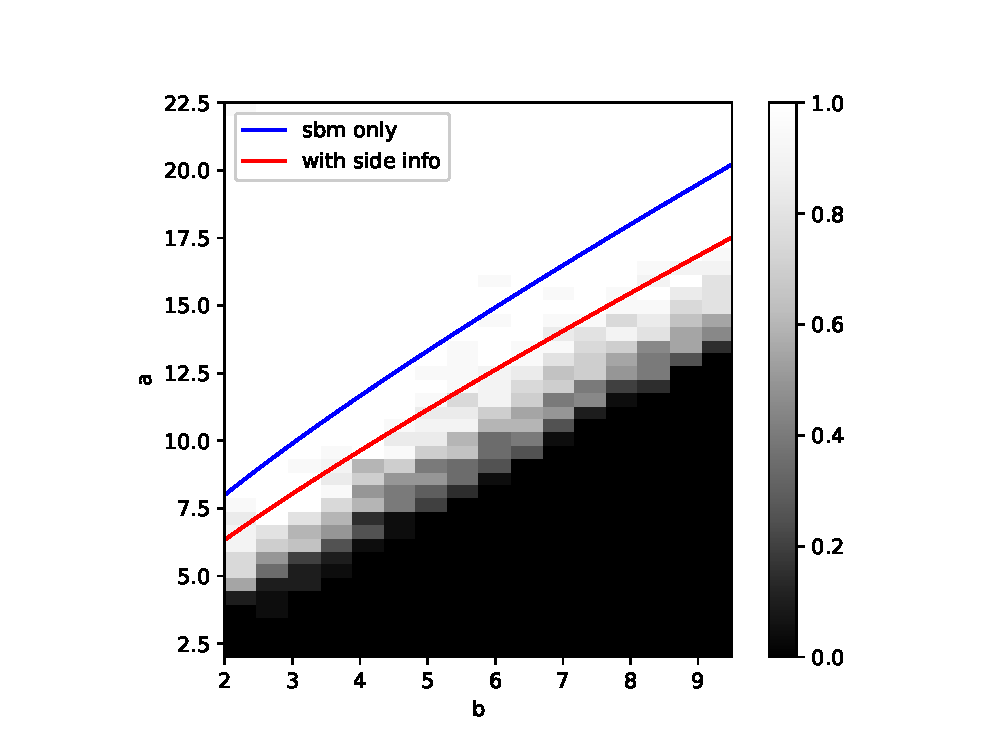
\includegraphics[width=0.6\textwidth]{sdp_si.eps}
	\caption{This plot shows that the empirical probability of successful recovery of the SDP algorithm 
	for the SBM with side information. We fix $n=300$ and the number of trials to be 20. The number of samples is chosen as $m=10$ for $\Bern(0.2)$ versus $\Bern(0.8)$. Then
	at each trial and for fixed $a$ and $b$, we check how many times each method succeeds. Dividing
	by the number of trials, we obtain the empirical probability of success with respect to
	the exact recovery metric. In blue, we plot the curve corresponding to the threshold $\sqrt{a}-\sqrt{b}=\sqrt{2}$ while in red we draw the curve corresponding to the threshold $\gamma D_{1/2}(p_0||p_1)  + (\sqrt{a} - \sqrt{b})^2 > 2$.}
\end{figure}

\subsection{Theoretical Guarantee}
We have already known that for $\kappa = \frac{\alpha \log n}{\beta n}$.
Actually we can relax $\kappa$ to a positive constant value.
Then the problem is to maximize
the following expression
\begin{equation}
\sum_{(i,j)\in E(G)} \sigma_i \sigma_j - \kappa \sum_{(i,j) \not\in E(G)} \sigma_i \sigma_j
\end{equation}
can be written in matrix form
as 
\begin{align}
\max \, & \sigma^T B \sigma \label{eq:sigmaB}\\
s.t. & \sigma_i \in \{\pm 1\} \notag
\end{align}
We can use semi-definite relaxation to solve this integer programming problems.
Let the matrix $B$ be defined as in \eqref{eq:B_matrix}.
Then we consider
\begin{align}
\max \,& Tr(BX) \label{eq:semiD}\\
s.t. & X_{ii} = 1 \notag \\
&  X \succeq 0 \notag
\end{align}
By following the same procedure in Abbe's paper \cite{abbe2015exact}, we can get the sufficient condition that the optimal solution
to \eqref{eq:semiD} is the ground truth vector $g$.
\begin{theorem}
If $\kappa > 0$ is a constant irrelevant with $n$, and $\sqrt{a} - \sqrt{b} > \sqrt{2}$, then for large enough $n$,
with high probability \eqref{eq:semiD} has a unique solution $g$.
\end{theorem}
The proof is similar with that of Abbe's paper \cite{abbe2015exact}.
We choose the conjugate vector $Y=\diag(Bgg^T)$ and show that 
 $Y \succeq B$ and $\lambda_2(Y-B)>0$.
$g$ is the eigenvector for $Y-B$, with the corresponding eigenvalue equal to zero.

We only need to show that $(g^{\perp})^T (Y-B)g^{\perp} >0$
for any vector $g^{\perp}$ perpendicular to $g$.

Using the following fact
\begin{align}
B &= (1+\kappa) A - \kappa(J_n - I_n) \\
\E[A] &= \frac{p-q}{2}gg^T + \frac{p+q}{2}J_n - pI_n
\end{align}
Then
\begin{align}
	(g^{\perp})^T(Y-B)g^{\perp} &= 
	(g^{\perp})^T\diag((1+\kappa)Agg^T) g^{\perp} 
	-(1+\kappa)(g^{\perp})^T(A-\E[A])g^{\perp}\notag\\
	&+p +(\kappa -(1+\kappa)\frac{p+q}{2})(g^{\perp})^TJ_ng^{\perp}
\end{align}
Since $\kappa -(1+\kappa)\frac{p+q}{2}>0$ for large $n$,
and there exists a constant $c>0$ such that with high
probability $\lambda_{\max}(A-\mathbb{E}[A]) \leq c\sqrt{\log n}$.
Then our task reduces to control
\begin{equation*}
	\min_{i} \{(Ag)_i g_i\} - c \sqrt{\log n} > 0
\end{equation*}
which is our familiar probability formulation.

Another proof is to decompose $Y-B=C-\Gamma$.
$C$ is a deterministic matrix
such that $\E[C]=\E[Y-B]$.
$\Gamma = Y-B-C$ satisfying $\E[\Gamma]=0$.

The modification of $\alpha_{ij}^+, \alpha_{ij}^-$ is as follows:
\begin{align}
\alpha^+_{ij}=\begin{cases} 1 & \text{wp }\A \\ -\kappa & \text{wp } 1-\A \end{cases}\\
\alpha^-_{ij}=\begin{cases} 1 & \text{wp }\B \\ -\kappa & \text{wp } 1-\B \end{cases}
\end{align}
The expression of $C, \Gamma$ are modified in corresponding way:
\begin{align}
C &=  \sum_{i<j, j \in S(i)}\left((1+\kappa)\A-\kappa\right)\Delta^+_{ij}+\sum_{i<j, j \notin S(i)} \left((1+\kappa)\B-\kappa\right) \Delta^-_{ij}\\
\Gamma &=  \sum_{i<j, j \in S(i)}\left(\left((1+\kappa)\A-\kappa\right) - \alpha^{+}_{ij}\right) \cdot \Delta^+_{ij} + \sum_{i<j, j \notin S(i)} \left(\left((1+\kappa)\B-\kappa\right) - \alpha^{-}_{ij}\right) \cdot \Delta^-_{ij}
\end{align}
$j\in S(i)$ means that $i,j$ belongs to the same community.

There is some minor problems when using projection in Abbe's paper. We can overcome the problem by consider
the event $\forall u \perp g, u^T(C-\Gamma)u \leq 0$, the probability of this event is bounded by
$$P(\min_{u \perp g, ||u||_2=1} u^T C u \leq \max_{||v||_2=1} v^T \Gamma v)$$.
For the determistic matrix $C$, we have
\begin{align}
a &= \kappa - (1+\kappa) \A \\
b &= \kappa - (1+\kappa) \B \\
d & = \kappa - (1+\kappa) \A + \frac{1+\kappa}{2} (a-b) \log n
\end{align}
Using Lemma \ref{lem:Cabd}, we can get all eigenvalues of $C$ as $\lambda_2=\frac{1+\kappa}{2}(a-b)\log n $ and $\lambda_1=n\kappa - (1+\kappa)b\log n$
(omit the eigenvalue corresponding to $g$). If $\kappa = 0$, then $C$ has negative eigenvalue and it is impossible for
$C-\Gamma \succeq 0 $ to hold
with large probability. The minimum requirement for this is that $\kappa > b\frac{\log n}{n}$.
This condition has been verified previously. Actually we need $\lambda_1 \geq \lambda_2$, and we obtain
$\kappa > \frac{a+b}{2} \frac{\log n}{n}$.

$\min_{u \perp g, ||u||_2=1} u^T C u = \min\{\lambda_1, \lambda_2\} := t$
Similar to the analysis in Section \ref{sec:original}, the non-diagonal term of the random matrix $\Gamma$ is $(1+\kappa)(A-E[A])$ and its
spectral norm is bounded by $c\sqrt{\log n}$ with large probability.
Therefore, we only need to consider the diagonal term of $\Gamma$, in which we have
$\Gamma_{ii} \geq \frac{1+\kappa}{2}(a-b)\log n \iff \sum_{j=1}^{n/2} z^-_{ij} - z^+_{ij} \geq 0$
where $z^-_{ij} \sim Bern(\B)$ and $z^+_{ij} \sim Bern(\A)$.
And we can get the threshold $\sqrt{a} - \sqrt{b} > \sqrt{2}$.

\section{SDP with $\{0,1\}$}
In this section, we consider the state taking values from $\{0,1\}$. Then using
the equivalent definition of $\delta(\sigma_i, \sigma_j) = \sigma_i \sigma_j + (1-\sigma_i)(1-\sigma_j)$ and
the equality $\sigma_i^2 =\sigma_i$
we can rewrite the object function
\begin{equation}
\sum_{(i,j)\in E(G)} \delta(\sigma_i, \sigma_j) -
\kappa \sum_{(i,j) \not\in E(G)} \delta(\sigma_i, \sigma_j)
\end{equation}
as $\sigma^T B \sigma$ where the matrix $B$ is defined as follows:
\begin{equation}
B_{ij} = \begin{cases}
1 & (i,j) \in E \\
-\kappa & (i,j) \not\in E\\
\kappa (n-1 - d_i) - d_i & i=j
\end{cases}
\end{equation}
where $d_i$ is the degree of the node $i$ in the graph.
All one vector is the eigenvector of the  matrix $B$ and its eigenvalue is zero.

%To simplify our discussion, we restrict our discussion on $\kappa = 1$.

We decompose the matrix $B$ into two parts, one part is $C$, a deterministic matrix and the other part is $\Gamma$, a random matrix
with zero expectation.
\begin{align}
B & = \sum_{i<j, j\in S(i)} \alpha_{ij}^+ \Delta_{ij} + \sum_{i<j, j\not\in S(i)}\alpha_{ij}^- \Delta_{ij} \\
& = C + \Gamma
\end{align}
where $\Delta_{ij} = -(e_i - e_j)(e_i - e_j)^T $.
The matrix $C$ and $\Gamma$ has the following form:
\begin{align*}
C &=  \sum_{i<j, j \in S(i)}\left((1+\kappa)\A-\kappa\right)\Delta_{ij}+\sum_{i<j, j \notin S(i)} \left((1+\kappa)\B-\kappa\right) \Delta_{ij}\\
\Gamma &=  \sum_{i<j, j \in S(i)}\left( \alpha^{+}_{ij} - \left((1+\kappa)\A-\kappa\right) \right) \cdot \Delta_{ij} + \sum_{i<j, j \notin S(i)} \left(\alpha^{-}_{ij}-\left((1+\kappa)\B-\kappa\right)\right) \cdot \Delta_{ij}
\end{align*}
We can compute the eigen-decomposition of $C$ using Lemma \ref{lem:Cabd}. The conclusion is that
$C$ has all-one eigenvector, with 0 as eigenvalue. $C$ also has an eigenvalue $\kappa n-(1+\kappa)b\log n$ with eigenvector $g$.
All other eigenvectors of $C$ belong to eigenvalue $n\kappa-\frac{1+\kappa}{2}(a+b)\log n $.

Now we relax to SDP problem, inspired by 3.1 of \cite{rendl2010semidefinite}.
That is, we consider an extension of $\tilde{B}$ of $(n+1)\times (n+1)$ dimension.
\begin{equation}
\tilde{B}_{ij} = \begin{cases}
B_{ij} & i,j\leq n \\
0 & \textrm{ otherwise}
\end{cases}
\end{equation}
Then we convert the problem to
\begin{align*}
\max\,& \tilde{B} \cdot X \\
s.t. & X_{ii} = X_{i,n+1} \textrm{ for } i = 1, \dots, n\\
& X_{n+1, n+1} = 1, X \succeq 0 \\
\end{align*}
By using Lagrange dual theorem, its dual problem can be written as:
\begin{align*}
\min \, & z \\
s.t.\, & \widetilde{T} = \begin{pmatrix}
2\diag(y) - B & -y \\
-y & z 
\end{pmatrix}\succeq 0
\end{align*}
where $y$ is a vector.


Let $g_1 = (0, 0 ,\dots, 0, 1, \dots, 1)$ be the vector corresponding to the ground truth.
We take $z = g_1^T B g_1$

Due to the symmetric property of the problem, if we should consider
$$
g_2 = (1, \dots, 1 ,0, \dots, 0)
$$
we have
\begin{equation}
g_1^T B g_1 = g_2^T B g_2 = -\sum_{i<j, j \not\in S(i)} B_{ij}
= -\sum_{i>j, j \not\in S(i)} B_{ij}
\end{equation}
since $B_{ij} = B_{ji}$ for $i\neq j$.

We should choose $y_i$ such that $\widetilde{T} \binom{g_1}{1} = 0 $ and $\widetilde{T} \binom{g_2}{1} = 0$.
$y_i = (Bg_2)_i$ for $i \leq \frac{n}{2}$ 
and
$y_i = -(Bg_1)_i$ for $i > \frac{n}{2}$.

Then we can verify that $y^T  g = 0$.

We first investigate the matrix $2\diag(y) - B$ and we define $z^* = 2E[y_i]= \kappa n - (1+\kappa)b\log n$.
Then
$2\diag(y)- B = C'-\Gamma'$
where
\begin{align}
C' &= z^* I - C \\
\Gamma' & =  \Gamma +  \diag\{z^* - 2y_1, \dots, z^* - 2y_n\} I 
\end{align}
Notice that $\Gamma'$ is a random matrix whose mean is zero.
For the deterministic matrix $C'$, it has eigenvalue $0$, eigenvector $g$;
eigenvalue $z^*$, eigenvector $\mathbf{1}$; eigenvalue $\frac{1+\kappa}{2}(a-b)\log n$ for other eigenvectors.

We can also verify that $g$ is the eigenvector of random matrix $\Gamma'$ since $(2\diag(y) - B)g=0$ ($\widetilde{T} \binom{g_1 - g_2}{0} = 0$).


Therefore, the condition $C' - \Gamma' \succeq 0$ is further equivalent to
\begin{equation}\label{eq:g1}
\frac{1+\kappa}{2}(a-b)\log n \geq u^T \Gamma' u, \forall ||u||_2 = 1, u \perp g
\end{equation}

We need to make sure that $z^* > \frac{1+\kappa}{2}(a-b)\log n$, which is approximately equivalent with
$\kappa > \frac{a+b}{2} \frac{\log n}{n}$.

The non-diagonal part of $\Gamma'$ is equal to $(1+\kappa)(A-E(A))$, whose spectral norm is $O(\sqrt{\log n})$.
Therefore, we only need to consider the diagonal term of $\Gamma'$ which is equal to guarantee:
$
\sum_{i=1}^{n/2} (X_i - Z_i) \geq \kappa
$ with large probability where $X_i \sim Bernoulli(\A), Z_i \sim Bernoulli(\B)$.
Thus, we have shown that $2\diag(y) - B \succeq 0$.

Then we use Cauchy Interlacing theorem to show that $\widetilde{T}$ is semi-positive definite.
% http://matrix.skku.ac.kr/Series-E/Monthly-E.pdf
Since $\widetilde{T}$ has at least two eigenvalues equal to 0, it must be the two smallest and our conclusion follows.

\section{Enhancement of Abbe's conclusion}\label{sec:original}
In Abbe's original formulation, he proposed a SDP algorithm which has theoretical
guarantee under a weak condition $(\alpha - \beta)^2 > 8(\alpha + \beta)$.
In this section, we show that this condition can be enhanced to $\sqrt{\alpha} - \sqrt{\beta} > \sqrt{2}$, which
is the detection threshold for SBM(2).
This result has already been obtained in Section 2 of \cite{hajek2016achieving}.

The key is to bound
$P(\lambda_{\max}(\Gamma) \geq (a-b)\log n)$,
we decompose the random matrix $\Gamma=\Gamma_1 +\Gamma_2$ to two parts: diagonal parts $\Gamma_1$ and non-diagonal parts $\Gamma_2$.
We can show that $\Gamma_2 = 2(A-E[A])$ where $A$ is the random adjacency matrix of the graph. It is a well known conclusion that
with probability $1-n^{-r}$ such that the spectral norm of $A-E[A]$ is bounded by $c\sqrt{\log n}$ (See Theorem 5.2 of \cite{lei2015consistency}).

By the property of spectral norm $||\Gamma_1 + \Gamma_2|| \leq ||\Gamma_1 || + ||\Gamma_2||$.
\begin{align*}
P(\lambda_{\max}(\Gamma) \geq (a-b)\log n) \leq & P(||\Gamma_1 || + ||\Gamma_2|| \geq (a-b) \log n)  \\
\leq & n^{-r} +
P(||\Gamma_1 || + ||\Gamma_2|| \geq (a-b) \log n, ||\Gamma_2||
\leq c\sqrt{\log n})\\
\leq & n^{-r} + P(||\Gamma_1|| \geq (a-b)\log n -c\sqrt{\log n}) \\
\leq & n^{-r} + \sum_{i=1}^n P(\Gamma_{ii} \geq (a-b)\log n -c\sqrt{\log n})
\end{align*}
Now we estimate $P(\Gamma_{11} \geq (a-b)\log n -c\sqrt{\log n})$, for the others are symmetric.
By some algebra we can get
$P(\Gamma_{11} \geq (a-b)\log n -c\sqrt{\log n}) = P(\sum_{i=1}^{n/2} z_i - x_i \geq -c\sqrt{\log n})$
where $z_i \sim Bern(\frac{\beta \log n}{n})$ and $x_i \sim Bern(\frac{\alpha \log n}{n})$.
This limit can be estimated as $(1+o(1))n^{-\frac{(\sqrt{\alpha}-\sqrt{\beta})^2}{2}}$.
Therefore, $P(\lambda_{\max}(\Gamma) \geq (a-b)\log n)\leq n^{-r} + (1+o(1))n^{1-\frac{(\sqrt{\alpha}-\sqrt{\beta})^2}{2}} = o(1)$
if $\sqrt{\alpha} - \sqrt{\beta} > \sqrt{2}$ is satisfied.
\section{SBM with multiple equal-sized clusters}
Using the notation of \cite{Hajek16}, we consider the SDP relation for SBM with multiple equal-sized clusters
\begin{align}
\max & \langle A,Z \rangle \notag \\
s.t. & Z \succeq 0, \notag\\
&Z_{ii} = 1,  && i \in [n] \notag\\
&Z_{ij} \geq 0, && i,j \in [n] \notag\\
&Z \mathbf{1} = K\mathbf{1} \label{eq:AZ}
\end{align}
where $K$ is the cluster size, $K=\frac{n}{k}$.
This method is called SDP-1 in \cite{amini2018semidefinite}.

Its dual problem can be written as:
\begin{align}
\min & \sum_{i=1}^n d_i + K \sum_{i=1}^n \lambda_i\notag \\
& D + \lambda \mathbf{1}^T - B - A \succeq 0, \textrm{ where } D=\diag(d_1, \dots, d_n), \lambda=(\lambda_1, \dots, \lambda_n) \notag \\
& B_{ij} \geq 0\label{eq:dualAZ}
\end{align}
When $Z^*$ is the optimal solution to \eqref{eq:AZ}, the optimal value for the primal problem is $\sum_{k=1}^r (\xi^*_k)^T A \xi^*_k
= \sum_{k=1}^r\sum_{i \in C_k} e(i, C_k) $. On the other hand, we choose
\begin{align}
d_i &= e(i, C_k) - r_i + 2\alpha_k  - \frac{1}{K} \sum_{i \in C_k} r_i \\
\lambda_i &= \frac{2}{K}(r_i - \alpha_k)
\end{align}
Then the optimal value for \eqref{eq:dualAZ} is also $\sum_{k=1}^r\sum_{i \in C_k} e(i, C_k) $.

We only need to verify $B, D, \lambda$ satisfy the constraint of \eqref{eq:dualAZ}.
$B$ is chosen by the following rule:
\begin{equation}
B_{ij} = \begin{cases}
0 & (i,j) \in C_k \textrm{ for some } k \\
y_{kk'}(i) + z_{kk'}(j) & \textrm{ where } i \in C_k, j \in C_{k'}
\end{cases}
\end{equation}
The intermediate parameter $y,z,\alpha,r_i$ can be defined properly.

\section{ML equivalent to min-cut}
In this section, we show that in $\SSBM(n,2,p,q)$,
ML is equivalent to solving the problem of minimum 2-cut,
.
Our starting point is the log likelihood function:
$$
L=\prod_{(i,j) \in E} p^{\delta(\sigma_i, \sigma_j)}q^{1-\delta(\sigma_i, \sigma_j)}
\prod_{(i,j)\not\in E} (1-p)^{\delta(\sigma_i, \sigma_j)}(1-q)^{1-\delta(\sigma_i, \sigma_j)}
$$
where $\sigma_i \in \{0,1\}$ and $\delta$ is the indicator function.
$\max \log L$ is equivalent to (neglecting some constant term for the given graph $G$)
$$
\max_{\sigma}
\log\frac{p}{q}\sum_{(i,j) \in E} \delta(\sigma_i, \sigma_j)
+\log \frac{1-p}{1-q}\sum_{(i,j)\not\in E} \delta(\sigma_i, \sigma_j)
$$
Using the fact that
$\sum_{(i,j) \in E}\delta(\sigma_i, \sigma_j)
+\sum_{(i,j)\not\in E} \delta(\sigma_i, \sigma_j)=\frac{n}{2}(\frac{n}{2}-1)$
we obtain
\begin{equation}\label{eq:sigma_tmp_max}
	\max_{\sigma} \log \frac{p(1-q)}{q(1-p)} \sum_{(i,j) \in E}\delta(\sigma_i, \sigma_j)
\end{equation}
Since $\log \frac{p(1-q)}{q(1-p)}>0$,
\eqref{eq:sigma_tmp_max} is equivalent to minimum 2-cut problem
\begin{equation}\label{eq:minimum_k_cut}
	\min \sum_{ \{i,j\} \in E} (1-\delta(x_i, x_j))
\end{equation}
\section{side information for SBM with k clusters}
There are $k$ labels: $\{1,2,\dots, k\}$.
Suppose each label $i$ corresponds to a distribution $P_i$.
The exact recovery condition: $I_+>1$.
where $I_+ = \min_{1\leq i < j \leq k} I_{ij}$.
$I_{ij}$ is defined in the following lemma
\begin{lemma}\label{lem:I_plus_expression}
	\begin{align}\label{equation:I+}
		I_{ij} &=\frac{\lambda^* }{k} (a^{1-\lambda^* }b^{\lambda^* } -
		b^{1-\lambda^* }a^{\lambda^* })\log\frac{b}{a}+\frac{a+b}{k}\notag \\
		&-\frac{1}{k}(a^{1-\lambda^*}b^{\lambda^*} +
		b^{1-\lambda^* }a^{\lambda^* })+\gamma D(P_{\lambda^* }||P_i) 
		\end{align}
		其中
		\begin{equation}\label{eq:lambda}
		\lambda^* = \arg\min_{\lambda} \left[a^{1-\lambda}b^{\lambda} +
		b^{1-\lambda}a^{\lambda} + k\gamma \log
		\left(\sum_{x\in \mathcal{X}}P^{1-\lambda}_i(x) P^{\lambda}_j(x)
		\right)
		\right]
	\end{equation}
	而 $P_{\lambda}$ 定义为
	\begin{equation}\label{eq:P_lambda_0_1}
		P_{\lambda}(x) = \frac{P_i^{1-\lambda}(x) P_j^{\lambda} (x)}
		{\sum_{x \in \mathcal{X}}P_i^{1-\lambda}(x) P_j^{\lambda} (x)}        
	\end{equation}
	
	\end{lemma}
	\begin{proof}
		We only need to let $c=\frac{a}{k}, d=\frac{b}{k}$ and
		compute the Chernoff Information between
		$\textrm{Pois}(c,d)\times \underbrace{P_i \times \dots \times P_i}_{\gamma}$
    and $\textrm{Pois}(d, c)\times \underbrace{P_j \times \dots \times P_j}_{\gamma}$.
	\end{proof}
	Below we give equivalent definition of $I_{ij}$.
	\begin{align}
		I_{ij} &=\min_{P_{\widetilde{Y}}}
		\gamma D(P_{\widetilde{Y}}|| P_i)
		+ \frac{1}{k} g(a,b, k\epsilon),
		\text{ 其中}\nonumber\\
		\epsilon &= \gamma \frac{D(P_{\widetilde{Y}} || P_j) - D(P_{\widetilde{Y}} || P_i) }{\log \frac{a}{b}}
   	\end{align}
\section{SBM, k communities, with side information}
Primal problem:
\begin{align}
\max & \langle \widetilde{B},X \rangle \notag \\
s.t. & X \succeq 0, \notag\\
&X_{ii} = 1,  && i \in [n] \notag\\
&X_{ij} \geq 0, && i,j \in [n] \notag\\
&\sum_{j=k+1}^{n+k} (X_{ij} + X_{ji})  = \frac{n}{k}&& \textrm{ for } i \in [n+k]\label{eq:AZ_ext}
\end{align}
The matrix $X$ is of size $(n+k) \times (n+k)$.
Suppose $\xi_i \in \{0,1\}^n $ is the true label vector for the $i$-th community.
and $\eta_i \in \{0,1\}^k$ is the indicator vector for the $i$-th community.
$|\xi_i|=n$ while $|\eta_i|=k$. Then we construct $g_i=(\eta_i, \xi_i)
\in \{0,1\}^{n+k}$.
The ground truth $X^*=\sum_{i=1}^k g_i g_i^T$.
The matrix $\widetilde{B}$ is constructed as
\begin{equation}\label{eq:B_lambda_def}
	\widetilde{B} = \begin{pmatrix} 0 & h^T  \\ h  & A \end{pmatrix}.
\end{equation}
$h$ is an $n\times k$ matrix, with entry $h_{ir} = \frac{1}{\log(a/b)}
\sum_{j=1}^m \log P_r(y^i_{j})$.
% and the matrix $B$ is defined in \eqref{eq:B_matrix}.


Let $S_1, \dots, S_k$ represent the community belonging set.
Then $[n]=\cup_{i=1}^k S_i$.

To simplify our analysis, we first consider $k=2$ and assume $S_1=\{1,2,\dots, n/2\}$ 
and $S_2=\{\frac{n}{2}+1, \dots, n\}$.

The following $(n+2)\times (n+2)$ matrix has two eigenvectors
$(1,0,\mathbf{1}_{n/2},0_{n/2})$,
$(0,1,0_{n/2},\mathbf{1}_{n/2})$
with eigenvalue 0.
\begin{align*}
	&\diag\{d_1^*, d_2^*, d_1, \dots, d_n\}
	-\begin{pmatrix}
		0 & b &  0_{n/2} & b'_1 \mathbf{1}_{n/2} \\
		b & 0 & b'_2 \mathbf{1}_{n/2} & 0_{n/2} \\
		0_{n/2} & b'_2 \mathbf{1}_{n/2} & 0 & B_{S_1 \times S_2} \\
		b'_1 b'_2 \mathbf{1}_{n/2} & 0_{n/2}& B_{S_1 \times S_2} & 0
	\end{pmatrix} \\
	&- \begin{pmatrix}
		0 & h^T \\
		h & A 
	\end{pmatrix}
	+ \begin{pmatrix}
		0 & 0 & b_1  \mathbf{1}^T_{n} \\
		0& 0 & b_2 \mathbf{1}^T_{n} \\
		b_1 \mathbf{1}_{n} & b_2 \mathbf{1}_{n}  & \lambda \mathbf{1}^T_{n} + \mathbf{1}_{n} \lambda^T
	\end{pmatrix}
\end{align*}
For $i\in [n/2]$, we have
\begin{align*}
	d_i &= \sum_{j=1}^{n/2} a_{ij}
	- \frac{n}{2} \lambda_i - \sum_{i=1}^{n/2} \lambda_i + h_{i1} - b_1 \\
	\frac{n}{2} \lambda_i &= \sum_{j=n/2 + 1}^{n} (B_{ij} + a_{ij} - \lambda_j) + b'_2 + h_{i2} - b_2
\end{align*}

For $n/2+1 \leq i \leq n$, we have
\begin{align*}
	d_i &= \sum_{j=n/2+1}^{n} a_{ij}
	- \frac{n}{2} \lambda_i - \sum_{i=n/2+1}^{n} \lambda_i + h_{i2} - b_2 \\
	\frac{n}{2} \lambda_i &= \sum_{j=1}^{n/2} (B_{ij} + a_{ij} - \lambda_j) + b'_1 + h_{i1} - b_1
\end{align*}

We make the following transformation:
\begin{equation*}
	\lambda_i = \begin{cases}
		\lambda'_i + \frac{h_{i2}}{n/2} & 1\leq i \leq n/2 \\
		\lambda'_i + \frac{h_{i1}}{n/2} & n/2+1 \leq i \leq n 
	\end{cases}
\end{equation*}
Then the above four equations are transformed to:


for $i\in [n/2]$,
\begin{align}
	d_i &= \sum_{j=1}^{n/2} a_{ij}
	- \frac{n}{2} \lambda'_i - \sum_{i=1}^{n/2} \lambda'_i + (h_{i1}- h_{i2}) - b_1 - \frac{1}{n/2}\sum_{i=1}^{n/2}h_{i2}
	\label{eq:lambda_prime_S_1}\\
	\frac{n}{2} \lambda'_i &= \sum_{j=n/2 + 1}^{n} (B_{ij} + a_{ij} - \lambda'_j) + b'_2 - b_2- \frac{1}{n/2}\sum_{i=n/2+1}^{n}h_{i1}
	\notag
\end{align}

for $n/2+1 \leq i \leq n$,
\begin{align}
	d_i &= \sum_{j=n/2+1}^{n} a_{ij}
	- \frac{n}{2} \lambda'_i - \sum_{i=n/2+1}^{n} \lambda'_i + (h_{i2} - h_{i1}) - b_2 -\frac{1}{n/2}\sum_{i=n/2+1}^{n}h_{i1}
	\label{eq:lambda_prime_S_2}\\
	\frac{n}{2} \lambda'_i &= \sum_{j=1}^{n/2} (B_{ij} + a_{ij} - \lambda'_j) + b'_1  - b_1- \frac{1}{n/2}\sum_{i=1}^{n/2}h_{i2}
	\notag
\end{align}

We also have the following four relationships:
\begin{align*}
d^*_1 - \sum_{i=1}^{n/2} h_{i1}	+ \frac{n}{2} b_1 & = 0\\
d^*_2 - \sum_{i=n/2+1}^{n} h_{i2} + \frac{n}{2} b_2 & = 0\\
-b - b'_1 \frac{n}{2} -  \sum_{i=n/2+1}^{n} h_{i1} + \frac{n}{2} b_1 & = 0\\
-b - b'_2 \frac{n}{2} -  \sum_{i=1}^{n/2} h_{i2} + \frac{n}{2} b_2 & = 0
\end{align*}
Therefore, we obtain:
\begin{equation*}
	b'_2 - b_2- \frac{1}{n/2}\sum_{i=n/2+1}^{n}h_{i1}
	=b'_1  - b_1- \frac{1}{n/2}\sum_{i=1}^{n/2}h_{i2}
	= \frac{-b}{n/2} - \frac{1}{n/2}
	\left(\sum_{i=1}^{n/2} h_{i2} + \sum_{i=n/2+1}^n h_{i1} \right)
\end{equation*}

We choose $b$ to make the above term vanish.
That is
\begin{equation*}
	b = -(\sum_{i \in S_1} h_{i2} + \sum_{i \in S_2}^n h_{i1} )
\end{equation*}
$b_1,b_2$ are chosen to make corresponding terms in \eqref{eq:lambda_prime_S_1},\eqref{eq:lambda_prime_S_2} vanish.
\begin{align*}
	b_1 &= - \frac{1}{n/2}\sum_{i \in S_1}h_{i2} \\
	b_2 &= - \frac{1}{n/2}\sum_{i \in S_2}h_{i1}
\end{align*}
Then $b'_1=b'_2=0$.

By Cauchy's interlacing theorem, we only need to show
the matrix $S^*=\diag\{d_1,\dots, d_n\} - B -A + \lambda \mathbf{1}^T_{n} + \mathbf{1}_{n} \lambda^T$ is positive definite.

\bibliographystyle{plain}
	\bibliography{exportlist.bib}
\end{document}